%! Date = 4/23/25
\section{Motivation}\label{sec:motivation}
\begin{figure}[!h]
    \centering
    \begin{subfigure}{0.425\textwidth}
        \centering
        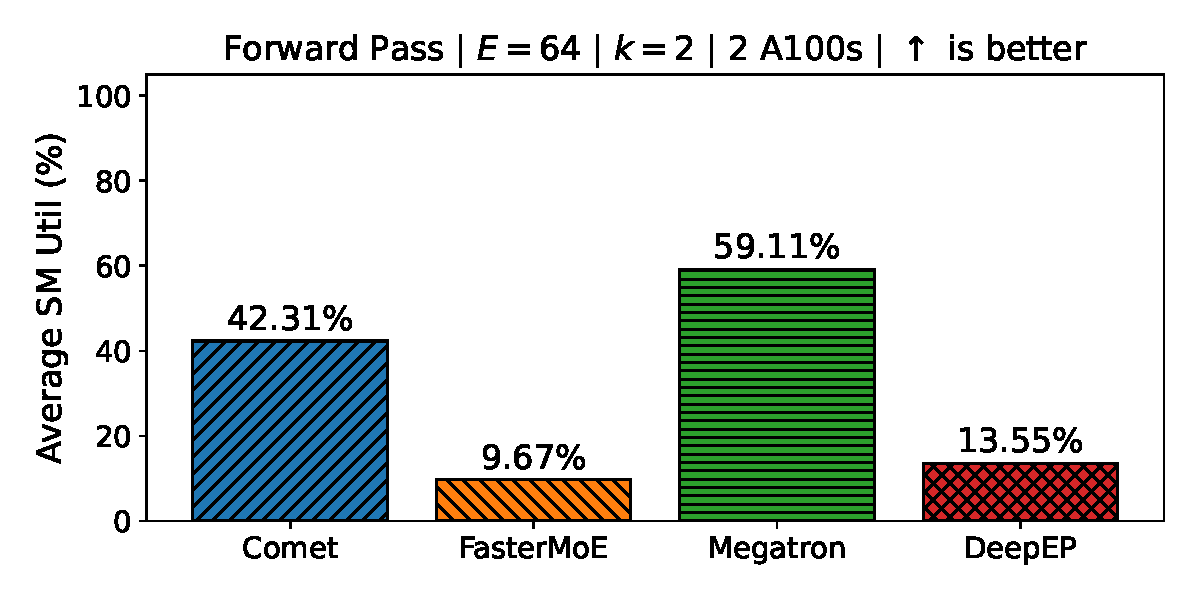
\includegraphics[width=\linewidth, keepaspectratio]{figures/sm_util_b}
        \caption{GPU SM Utilization across baselines}
        \label{sub:util}
    \end{subfigure}
    \begin{subfigure}{0.425\textwidth}
        \centering
        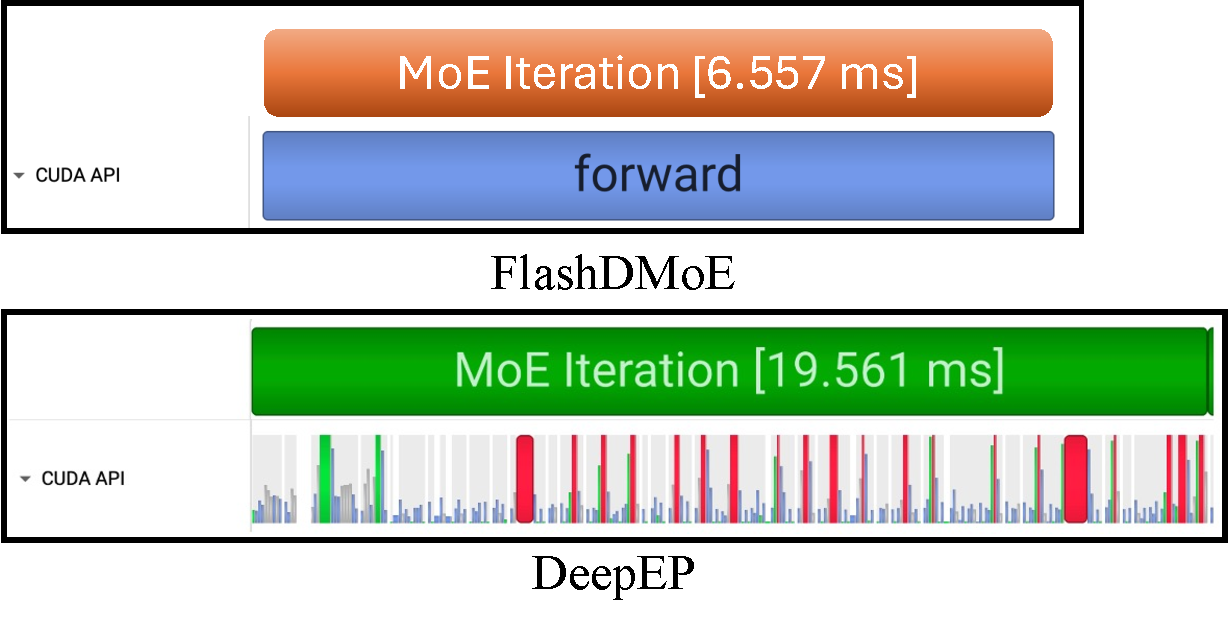
\includegraphics[width=\textwidth, keepaspectratio]{figures/kernel_launch}
        \caption{Kernel Launch overhead (CUDA API row)}
        \label{sub:launch}
    \end{subfigure}
    \caption{\ref{sub:util} shows GPU utilization averaged across 100 MoE forward passes on 2 A100s with
    300 GB/s unidirectional bandwidth, where we observe up to 90\% idle time, due to kernel launch gaps and
    non-overlapping communication.}
    \label{fig:kl}
\end{figure}
\myparab{Synchronous Communication.} \emph{AlltoAll} or \emph{AllGather} communication as currently used in MoE frameworks
is a \emph{synchronous} collective operation, whose completion requires the participation of all involved GPUs.
Here, disparities in processing speeds or kernel scheduling
among GPUs induce a straggler effect detrimental (Figure~\ref{fig:overlap}) to (1) the collective operation's performance and (2)
E2E performance, as stalled GPUs cannot proceed to downstream dependent or independent tasks until the collective terminates.
We expound on this problem in~\S\ref{sec:motivation-appx}.

\myparab{Kernel Launch Overhead.} We compare the kernel launch overheads between \sysname and existing baselines.
Table~\ref{tab:gpuOps} shows the number of kernel launches during a single forward pass: \sysname launches exactly one persistent kernel, while the baselines launch up to 550 short-lived kernels to perform the same computation.
Figure~\ref{fig:kl} provides a visual comparison using CUDA API traces captured by NSight Systems, illustrating the difference between \sysname and DeepEP.
DeepEP exhibits many small CUDA API calls, with frequent stalls between individual operators, leading to increased GPU idle time (Figure~\ref{sub:util}).
In contrast, \sysname maintains high GPU utilization by avoiding launch overhead and synchronization gaps—achieving \textbf{93.17}\%
GPU utilization compared to 14\% for DeepEP. See \S\ref{sec:evaluation} for experimental results and \S\ref{sec:related}
for a discussion of related work.